%%%%%%%%%%%%%%%%%%%%%%%%%%%%%%%%%%%%%%%%%
% Beamer Presentation
% LaTeX Template
% Version 2.0 (March 8, 2022)
%
% This template originates from:
% https://www.LaTeXTemplates.com
%
% Author:
% Vel (vel@latextemplates.com)
%
% License:
% CC BY-NC-SA 4.0 (https://creativecommons.org/licenses/by-nc-sa/4.0/)
%
%%%%%%%%%%%%%%%%%%%%%%%%%%%%%%%%%%%%%%%%%

%----------------------------------------------------------------------------------------
%	PACKAGES AND OTHER DOCUMENT CONFIGURATIONS
%----------------------------------------------------------------------------------------

\documentclass[
	10pt, % Set the default font size, options include: 8pt, 9pt, 10pt, 11pt, 12pt, 14pt, 17pt, 20pt
	%t, % Uncomment to vertically align all slide content to the top of the slide, rather than the default centered
	aspectratio=169, % Uncomment to set the aspect ratio to a 16:9 ratio which matches the aspect ratio of 1080p and 4K screens and projectors
]{beamer}

\usepackage[all]{xy}

\usepackage[spanish]{babel}
\usepackage[utf8]{inputenc}

\graphicspath{{Images/}{./}} % Specifies where to look for included images (trailing slash required)

\usepackage{booktabs} % Allows the use of \toprule, \midrule and \bottomrule for better rules in tables

%\usepackage{tikz}
%\usetikzlibrary{positioning}
%\usetikzlibrary{shapes,arrows,arrows,positioning,fit}

\usepackage{tikz}
\usetikzlibrary{mindmap}

\usepackage{multirow}

\usepackage{graphicx}
\usepackage{hyperref}

\usepackage{venndiagram}

\usepackage{xcolor,listings}
\usepackage{textcomp}
\usepackage{color}

\usepackage{enumitem}

\usepackage{array}
\usepackage{verbatim}

\usepackage[inkscapeformat=png]{svg}

\definecolor{codegreen}{rgb}{0,0.6,0}
\definecolor{codegray}{rgb}{0.5,0.5,0.5}
\definecolor{codepurple}{HTML}{C42043}
\definecolor{backcolour}{HTML}{F2F2F2}
\definecolor{red}{HTML}{FF0000}
\definecolor{bookColor}{cmyk}{0,0,0,0.90}  
\color{bookColor}

\lstset{upquote=true}

\lstdefinestyle{mystyle}{
	backgroundcolor=\color{backcolour},   
	commentstyle=\color{codegreen},
	keywordstyle=\color{codepurple},
	numberstyle=\numberstyle,
	stringstyle=\color{codepurple},
	basicstyle=\footnotesize\ttfamily,
	breakatwhitespace=false,
	breaklines=true,
	captionpos=b,
	keepspaces=true,
	numbers=left,
	numbersep=10pt,
	showspaces=false,
	showstringspaces=false,
	showtabs=false,
	otherkeywords = {OUT, SIGNAL, DECLARE, BEFORE, AFTER, CALL, WHILE, PROCEDURE},
}
\lstset{style=mystyle}

\newcommand\numberstyle[1]{%
	\footnotesize
	\color{codegray}%
	\ttfamily
	\ifnum#1<10 0\fi#1 |%
}


%----------------------------------------------------------------------------------------
%	SELECT LAYOUT THEME
%----------------------------------------------------------------------------------------

% Beamer comes with a number of default layout themes which change the colors and layouts of slides. Below is a list of all themes available, uncomment each in turn to see what they look like.

%\usetheme{default}
%\usetheme{AnnArbor}
%\usetheme{Antibes}
%\usetheme{Bergen}
%\usetheme{Berkeley}
%\usetheme{Berlin}
%\usetheme{Boadilla} % interesante
%\usetheme{CambridgeUS}
%\usetheme{Copenhagen}
%\usetheme{Darmstadt}
%\usetheme{Dresden}
%\usetheme{Frankfurt}
%\usetheme{Goettingen}
%\usetheme{Hannover}
%\usetheme{Ilmenau}
%\usetheme{JuanLesPins}
%\usetheme{Luebeck}
\usetheme{Madrid} % interesante
%\usetheme{Malmoe}
%\usetheme{Marburg}
%\usetheme{Montpellier}
%\usetheme{PaloAlto}
%\usetheme{Pittsburgh} % interesante
%\usetheme{Rochester} % interesante este
%\usetheme{Singapore}
%\usetheme{Szeged}
%\usetheme{Warsaw}

%----------------------------------------------------------------------------------------
%	SELECT COLOR THEME
%----------------------------------------------------------------------------------------

% Beamer comes with a number of color themes that can be applied to any layout theme to change its colors. Uncomment each of these in turn to see how they change the colors of your selected layout theme.

%\usecolortheme{albatross}
%\usecolortheme{beaver}
%\usecolortheme{beetle}
%\usecolortheme{crane}
%\usecolortheme{dolphin}
%\usecolortheme{dove}
%\usecolortheme{fly}
%\usecolortheme{lily}
%\usecolortheme{monarca}
%\usecolortheme{seagull}
%\usecolortheme{seahorse}
%\usecolortheme{spruce} % verde suave
%\usecolortheme{whale}
%\usecolortheme{wolverine}

%----------------------------------------------------------------------------------------
%	SELECT FONT THEME & FONTS
%----------------------------------------------------------------------------------------

% Beamer comes with several font themes to easily change the fonts used in various parts of the presentation. Review the comments beside each one to decide if you would like to use it. Note that additional options can be specified for several of these font themes, consult the beamer documentation for more information.

\usefonttheme{default} % Typeset using the default sans serif font
%\usefonttheme{serif} % Typeset using the default serif font (make sure a sans font isn't being set as the default font if you use this option!)
%\usefonttheme{structurebold} % Typeset important structure text (titles, headlines, footlines, sidebar, etc) in bold
%\usefonttheme{structureitalicserif} % Typeset important structure text (titles, headlines, footlines, sidebar, etc) in italic serif
%\usefonttheme{structuresmallcapsserif} % Typeset important structure text (titles, headlines, footlines, sidebar, etc) in small caps serif

%------------------------------------------------

%\usepackage{mathptmx} % Use the Times font for serif text
%\usepackage{palatino} % Use the Palatino font for serif text

\usepackage{helvet} % Use the Helvetica font for sans serif text
%\usepackage[default]{opensans} % Use the Open Sans font for sans serif text
%\usepackage[default]{FiraSans} % Use the Fira Sans font for sans serif text
\usepackage[default]{lato} % Use the Lato font for sans serif text

%----------------------------------------------------------------------------------------
%	SELECT INNER THEME
%----------------------------------------------------------------------------------------

% Inner themes change the styling of internal slide elements, for example: bullet points, blocks, bibliography entries, title pages, theorems, etc. Uncomment each theme in turn to see what changes it makes to your presentation.

%\useinnertheme{default}
\useinnertheme{circles}
%\useinnertheme{rectangles}
%\useinnertheme{rounded}
%\useinnertheme{inmargin}

%----------------------------------------------------------------------------------------
%	SELECT OUTER THEME
%----------------------------------------------------------------------------------------

% Outer themes change the overall layout of slides, such as: header and footer lines, sidebars and slide titles. Uncomment each theme in turn to see what changes it makes to your presentation.

%\useoutertheme{default}
%\useoutertheme{infolines}
%\useoutertheme{miniframes}
%\useoutertheme{smoothbars}
%\useoutertheme{sidebar}
%\useoutertheme{split}
%\useoutertheme{shadow}
%\useoutertheme{tree}
%\useoutertheme{smoothtree}

\setbeamertemplate{footline} % Uncomment this line to remove the footer line in all slides
%\setbeamertemplate{footline}[page number] % Uncomment this line to replace the footer line in all slides with a simple slide count

\setbeamertemplate{navigation symbols}{} % Uncomment this line to remove the navigation symbols from the bottom of all slides

%----------------------------------------------------------------------------------------
%	PRESENTATION INFORMATION
%----------------------------------------------------------------------------------------

\title[Short Title]{Bases de Datos I} % The short title in the optional parameter appears at the bottom of every slide, the full title in the main parameter is only on the title page

\subtitle{Disparadores y procedimientos almacenados en SQL} % Presentation subtitle, remove this command if a subtitle isn't required

\author{Lic. Carlos León González \\ Dra.C. Lucina García Hernández} % Presenter name(s), the optional parameter can contain a shortened version to appear on the bottom of every slide, while the main parameter will appear on the title slide

\institute[UC]{Facultad de Matemática y Computación \\ Universidad de La Habana \\ \smallskip} % Your institution, the optional parameter can be used for the institution shorthand and will appear on the bottom of every slide after author names, while the required parameter is used on the title slide and can include your email address or additional information on separate lines

\date[\today]{\today} % Presentation date or conference/meeting name, the optional parameter can contain a shortened version to appear on the bottom of every slide, while the required parameter value is output to the title slide

%----------------------------------------------------------------------------------------

\begin{document}

\lstset{
	literate=%
	{á}{{\'a}}1
	{í}{{\'i}}1
	{é}{{\'e}}1
	{ý}{{\'y}}1
	{ú}{{\'u}}1
	{ó}{{\'o}}1
	{ě}{{\v{e}}}1
	{š}{{\v{s}}}1
	{č}{{\v{c}}}1
	{ř}{{\v{r}}}1
	{ž}{{\v{z}}}1
	{ď}{{\v{d}}}1
	{ť}{{\v{t}}}1
	{ň}{{\v{n}}}1                
	{ů}{{\r{u}}}1
	{Á}{{\'A}}1
	{Í}{{\'I}}1
	{É}{{\'E}}1
	{Ý}{{\'Y}}1
	{Ú}{{\'U}}1
	{Ó}{{\'O}}1
	{Ě}{{\v{E}}}1
	{Š}{{\v{S}}}1
	{Č}{{\v{C}}}1
	{Ř}{{\v{R}}}1
	{Ž}{{\v{Z}}}1
	{Ď}{{\v{D}}}1
	{Ť}{{\v{T}}}1
	{Ň}{{\v{N}}}1                
	{Ů}{{\r{U}}}1    
}

%----------------------------------------------------------------------------------------
%	TITLE SLIDE
%----------------------------------------------------------------------------------------

\begin{frame}
	\titlepage % Output the title slide, automatically created using the text entered in the PRESENTATION INFORMATION block above
\end{frame}

%------------------------------------------------

{
	\setbeamertemplate{background canvas}
	{%
		
\includegraphics[width=\paperwidth,height=\paperheight]{sql+.jpeg}
	}
	
	\begin{frame}
	\end{frame}
}

%------------------------------------------------

\begin{frame}{t}
	
	\frametitle{Problema}
	
	Supongamos que existe una tabla llamada ``Pedido'' que almacena información sobre los clientes. Cada vez que se inserta un nuevo pedido en esta tabla, también se desea actualizar \textcolor<2>{red}{automáticamente} la tabla ``Inventario'' para reflejar la disminución de existencias de los productos.
	
\end{frame}

%------------------------------------------------

\begin{frame}{t}
	
	\frametitle{Solución}
	
	\begin{enumerate}
		
		\item Junto a la instrucción \textcolor{codepurple}{INSERT}, mandarle al SGBD una instrucción \textcolor{codepurple}{UPDATE}. \only<3>{No son operaciones automáticas, sino manuales.}
		
		\ 
		
		\  
		
		\only<2>{Esta propuesta no soluciona el requisito de ser una operación \textcolor{red}{automática}}
		
		\pause
		\item<3> Usar un disparador.
		
	\end{enumerate}
	
\end{frame}

%------------------------------------------------

\begin{frame}{t}
	
	\frametitle{Características de un disparador (\emph{trigger})}
	
	\begin{itemize}
		
		\item Es un procedimiento que se activa automáticamente sobre una tabla asociada previamente
		
		\pause
		\item Los posibles eventos que activan el \emph{trigger} son aquellas operaciones que modifican el estado de la tabla, o sea: 
			\begin{itemize}
				\item \textcolor{codepurple}{INSERT}
				\item \textcolor{codepurple}{UPDATE}
				\item \textcolor{codepurple}{DELETE}
			\end{itemize}
			
		\pause
		\item No requiere intervención humana o programática para ejecutarse y no se puede detener una vez activado
		
		\pause
		\item Se utiliza para garantizar el cumplimiento de ciertas reglas del negocio y modificar los valores de los atributos de forma dinámica
		
	\end{itemize}	
	
\end{frame}

%------------------------------------------------

\begin{frame}[fragile]
	
	\frametitle{Ventajas de los \emph{triggers}}
	
	Este recurso brindado por SQL, brinda al programador a:
	
	\begin{itemize}
		
		\item Realizar cambios en cascada en la base de datos
		
		\pause 
		
		\item Comprobar restricciones más complejas que las definidas en el \textcolor{codepurple}{CHECK}
		
		\pause
		
		\item Evaluar el estado de una tabla antes y después de realizar una modificación de datos y actuar en función de la diferencia utilizando \textcolor{codepurple}{NEW} and \textcolor{codepurple}{OLD}
		
		\pause
		
		\item Tratar errores de manera más personalizada y compleja
		
	\end{itemize}

\end{frame}

%------------------------------------------------

\begin{frame}[fragile]
	
	\frametitle{Contexto de ejecución de dos \emph{triggers}}
	
	\begin{figure}[h]
		\centering
		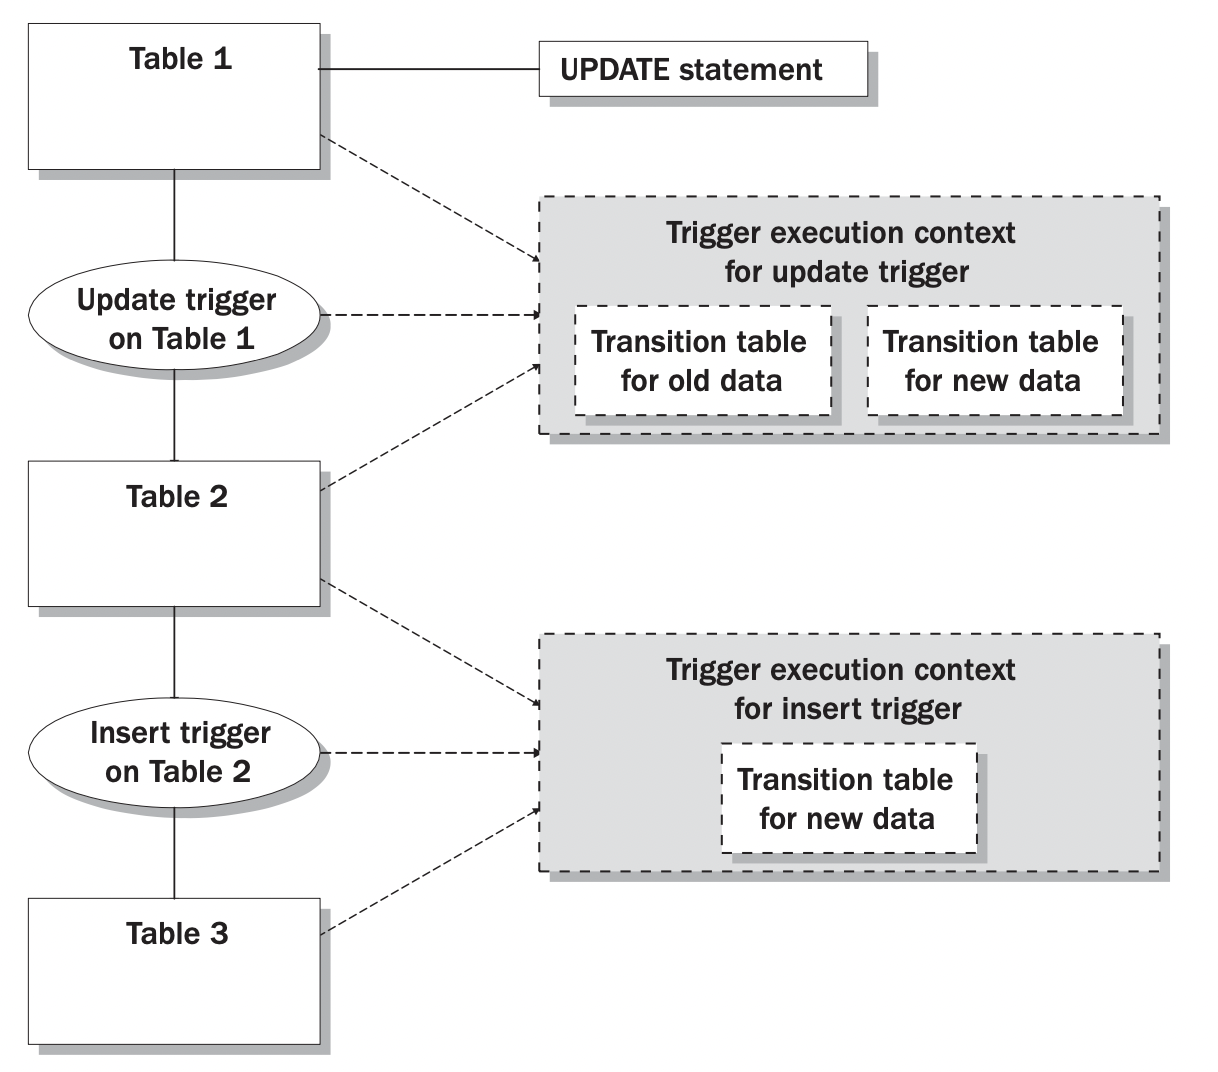
\includegraphics[scale=0.4]{flujo-trigger.png}
	\end{figure}

\end{frame}

%------------------------------------------------

\begin{frame}[fragile]
	
	\frametitle{Sintaxis de los \emph{triggers}}
	
	\begin{lstlisting}[ language=SQL,
		deletekeywords={IDENTITY},
		deletekeywords={[2]INT},
		morekeywords={clustered},
		framesep=8pt,
		xleftmargin=40pt,
		framexleftmargin=40pt,
		frame=tb,
		framerule=0pt ]
CREATE TRIGGER <trigger_name> <trigger_order> <trigger_event> 
ON <table_name> 
FOR EACH ROW <trigger_statement>;
\end{lstlisting}

	\ 
	
	\ 
	
	\pause
	
	El campo \texttt{<trigger\_order>} define el momento en que se ejecuta/activa un \emph{trigger}:
	
	\begin{itemize}
		
		\item \textcolor{codepurple}{BEFORE} 
		\\ Antes de ejecutarse la cláusula definida
		
		\item \textcolor{codepurple}{AFTER} 
		\\ Posterior a la ejecución de la cláusula definida
		
	\end{itemize}
	
\end{frame}

%------------------------------------------------

\begin{frame}[fragile]
	
	\frametitle{Sintaxis de los \emph{triggers}}
	
	\begin{lstlisting}[ language=SQL,
		deletekeywords={IDENTITY},
		deletekeywords={[2]INT},
		morekeywords={clustered},
		framesep=8pt,
		xleftmargin=40pt,
		framexleftmargin=40pt,
		frame=tb,
		framerule=0pt ]
CREATE TRIGGER <trigger_name> <trigger_order> <trigger_event> 
ON <table_name> 
FOR EACH ROW <trigger_statement>;
\end{lstlisting}
	
	\ 
	
	\ 
	
	\pause
	
	El campo \texttt{<trigger\_event>} establece el evento sobre el cual se define el \emph{trigger}. Solo pueden definirse cláusulas que modifican el estado de los registros de la base de datos. 
	
	\pause
	
	\begin{table}[]
		\begin{tabular}{| c | c | c |}
			\hline
			Evento & Acceso a la variable \textcolor{codepurple}{NEW} & Acceso a la variable \textcolor{codepurple}{OLD} \\ \hline \hline
			\textcolor{codepurple}{INSERT} & Sí, representa la tupla a insertar & No \\ \hline
			\textcolor{codepurple}{DELETE} & No & Sí, representa la tupla antes de eliminarla \\ \hline
			\textcolor{codepurple}{UPDATE} & Sí, representa la tupla después de editarla & Sí, representa la tupla antes de editarla \\ \hline
		\end{tabular}
	\end{table}
	
\end{frame}

%------------------------------------------------

\begin{frame}[fragile]
	
	\frametitle{Sintaxis de los \emph{triggers}}
	
	\begin{lstlisting}[ language=SQL,
		deletekeywords={IDENTITY},
		deletekeywords={[2]INT},
		morekeywords={clustered},
		framesep=8pt,
		xleftmargin=40pt,
		framexleftmargin=40pt,
		frame=tb,
		framerule=0pt ]
CREATE TRIGGER <trigger_name> <trigger_order> <trigger_event> 
ON <table_name> 
FOR EACH ROW <trigger_statement>;
\end{lstlisting}

	\ 
	
	\pause
	
	La expresión \texttt{<trigger\_statement>} permite utilizar instrucciones de la programación imperativa y combinarla con las siguientes instrucciones declarativas: 
	\begin{columns}[t]
		\column{0.3\textwidth}
		
		\begin{itemize}
			\item \textcolor{codepurple}{INSERT}
			\item \textcolor{codepurple}{UPDATE}
			\item \textcolor{codepurple}{DELETE}
		\end{itemize}
		
		\column{0.3\textwidth}
		
		\begin{itemize}
			\item \textcolor{codepurple}{CREATE}
			\item \textcolor{codepurple}{DROP}
			\item \textcolor{codepurple}{ALTER}
		\end{itemize}
		
		\column{0.3\textwidth}
		
		\begin{itemize}
			\item \textcolor{codepurple}{SELECT}
		\end{itemize}
		
	\end{columns}
	
	\ 
	
	\ 
	
	\pause
	
	Estructura: 
		\begin{lstlisting}[ language=SQL,
		deletekeywords={IDENTITY},
		deletekeywords={[2]INT},
		morekeywords={clustered},
		framesep=8pt,
		xleftmargin=40pt,
		framexleftmargin=40pt,
		frame=tb,
		framerule=0pt ]
BEGIN
<body>
END;
\end{lstlisting}
	
\end{frame}

%------------------------------------------------

\begin{frame}[fragile]
	
	\frametitle{Algunas instrucciones imperativas}
	
	\begin{columns}[t]
		\column{0.5\textwidth}
		
			\begin{itemize}
			
			\item Declaración de variables \\
			\texttt{\textcolor{codepurple}{DECLARE} <var\_name> <var\_type>} \\ 
			\texttt{\textcolor{codepurple}{@}<var\_name>}
			
			\pause
			\ 
			
			\item  Asignación de valor \\ 
			\texttt{\textcolor{codepurple}{SET} <var\_name> = <value>}
			
			\pause
			\ 
			
			\item  Uso de condiciones \\
			\texttt{\textcolor{codepurple}{IF} <conditional\_expression> \\ 
				\textcolor{codepurple}{THEN} <statements\_block> \\ 
				\textcolor{codepurple}{ELSE} <statements\_block> \\ 
				\textcolor{codepurple}{END IF}}
			
		\end{itemize}
		
		\column{0.5\textwidth}
		
			\begin{itemize}
				
			\pause 
						
			\item Uso de ciclos (WHILE / DO-WHILE)\\
			\texttt{\textcolor{codepurple}{WHILE}  <conditional\_expression>  \\
			\textcolor{codepurple}{DO}  <statements\_block> \\
			\textcolor{codepurple}{END WHILE}} \\
			
			\ 
			
			\texttt{\textcolor{codepurple}{REPEAT}  <statements\_block>  \\
			\textcolor{codepurple}{UNTIL} <conditional\_expression> \\
			\textcolor{codepurple}{END REPEAT}}
			
			\pause
			\ 
			
			\item Detener ciclos (BREAK)\\ 
			\texttt{\textcolor{codepurple}{LEAVE}}
			
		\end{itemize}
		
	\end{columns}
	
\end{frame}

%------------------------------------------------

\begin{frame}{t}
	
	\frametitle{Recordando nuestra base de datos}
	
	\begin{figure}[h]
		\centering
		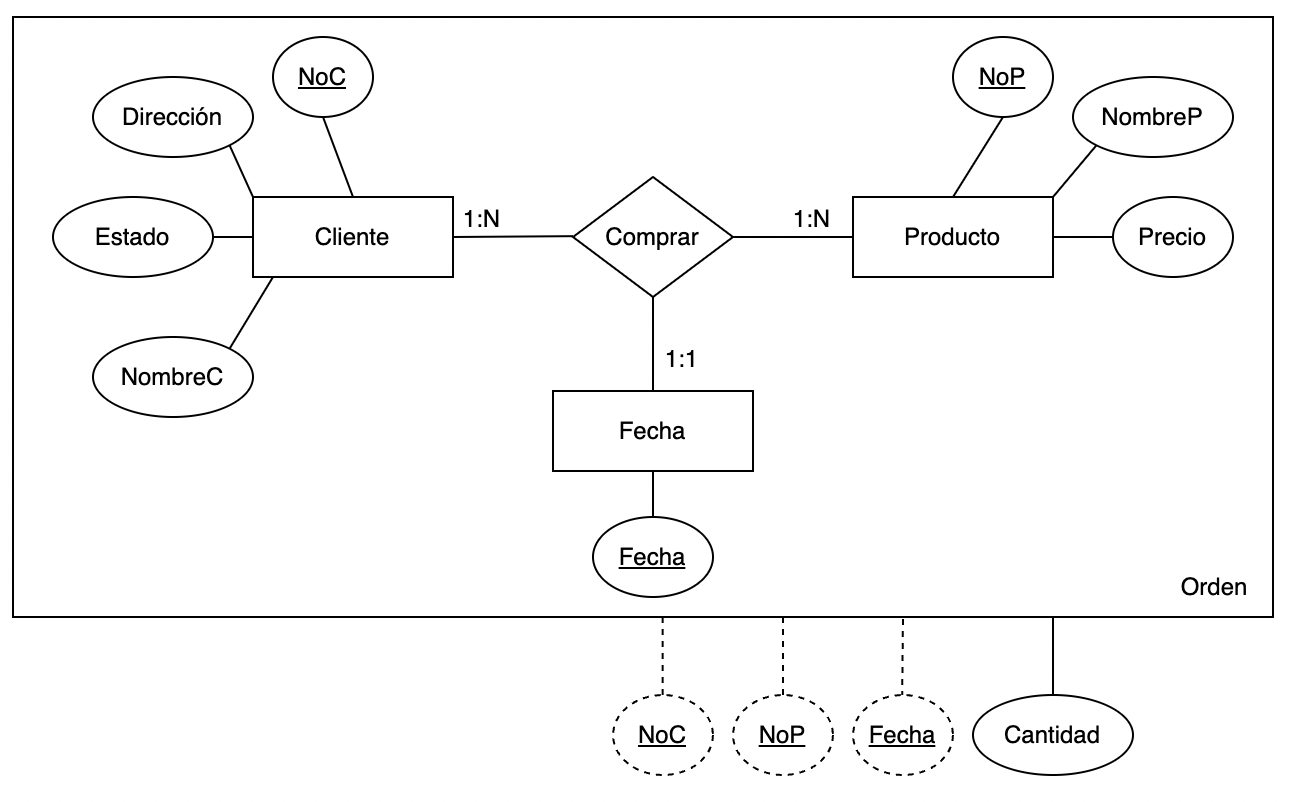
\includegraphics[scale=0.5]{bd.png}
	\end{figure}
	
	
\end{frame}

%------------------------------------------------

\begin{frame}[fragile]
	
	\frametitle{Ejemplo}
	
	Problema: \\
	Construya un \emph{trigger} para limitar la cantidad de unidades por producto, en una orden de compra. Cada producto tiene definido el máximo de compras por día.
	
	\ 
	
	Solución: \\
	
	\begin{onlyenv}<1-2>
		\begin{lstlisting}[ language=SQL,
			deletekeywords={IDENTITY},
			deletekeywords={[2]INT},
			morekeywords={clustered},
			framesep=8pt,
			xleftmargin=40pt,
			framexleftmargin=40pt,
			frame=tb,
			framerule=0pt ]
CREATE TRIGGER trg_limit_test <trigger_order> <trigger_event> 
ON <table_name> 
FOR EACH ROW <trigger_statement>;
\end{lstlisting}
	\end{onlyenv}

	\begin{onlyenv}<3-4>
		\begin{lstlisting}[ language=SQL,
			deletekeywords={IDENTITY},
			deletekeywords={[2]INT},
			morekeywords={clustered},
			framesep=8pt,
			xleftmargin=40pt,
			framexleftmargin=40pt,
			frame=tb,
			framerule=0pt ]
CREATE TRIGGER <trigger_name> <trigger_order> <trigger_event> 
ON Orden
FOR EACH ROW <trigger_statement>;
\end{lstlisting}
	\end{onlyenv}
	
	\begin{onlyenv}<5-6>
		\begin{lstlisting}[ language=SQL,
			deletekeywords={IDENTITY},
			deletekeywords={[2]INT},
			morekeywords={clustered},
			framesep=8pt,
			xleftmargin=40pt,
			framexleftmargin=40pt,
			frame=tb,
			framerule=0pt ]
CREATE TRIGGER <trigger_name> BEFORE INSERT 
ON orden
FOR EACH ROW <trigger_statement>;
\end{lstlisting}
	\end{onlyenv}
	
		\begin{onlyenv}<7>
		\begin{lstlisting}[ language=SQL,
			deletekeywords={IDENTITY},
			deletekeywords={[2]INT},
			morekeywords={clustered},
			framesep=8pt,
			xleftmargin=40pt,
			framexleftmargin=40pt,
			frame=tb,
			framerule=0pt ]
CREATE TRIGGER <trigger_name> BEFORE INSERT 
ON Orden
FOR EACH ROW BEGIN

  -- (1) Dado el cliente (NEW.NoC), obtener la cantidad de productos igual al comprado (NEW.NoP), adquiridos en la fecha actual (NEW.Fecha)
  
  -- (2) Obtener el límite de productos del tipo NEW.NoP, que se puede adquirir en un mismo día
  
  -- (3) Verificar si la cantidad de productos comprados, más la almacenada, supera la cantidad límite

END;
\end{lstlisting}
\end{onlyenv}
		
	\ 
	
	\ 
	
	\only<2>{\textcolor{red}{¿Sobre qué relación trabajará el \emph{trigger}?}}
	
	\only<4>{\textcolor{red}{¿Con el uso de qué clásula se activará el \emph{trigger}? ¿Cuándo lo hará?}}
	
	\only<6>{\textcolor{red}{¿Qué debe de hacer el \emph{trigger}?}}
	
\end{frame}

%------------------------------------------------

\begin{frame}[fragile]
	
	\frametitle{Ejemplo - Solución}
	
	\begin{lstlisting}[ language=SQL,
		deletekeywords={IDENTITY},
		deletekeywords={[2]INT},
		morekeywords={clustered},
		framesep=8pt,
		xleftmargin=40pt,
		framexleftmargin=40pt,
		frame=tb,
		framerule=0pt ]
CREATE TRIGGER trg_limit_test BEFORE INSERT 
ON Orden
FOR EACH ROW BEGIN
  DECLARE total INT;
  DECLARE limiteDiario INT;
  -- (1) 
  SET total = (
    SELECT SUM(Cantidad) 
    FROM orden 
    WHERE NoC = NEW.NoC AND NoP = NEW.NoP AND DATE(Fecha) = DATE(NEW.Fecha)
  );
  -- (2)
  SET limiteDiario = (
    SELECT MIN(producto.LimiteDiario) 
    FROM producto 
    WHERE producto.NoP = NEW.NoP
  );
  -- (3)
  IF total + NEW.Cantidad > limiteDiario THEN
    SIGNAL SQLSTATE '45000' SET MESSAGE_TEXT = 'Acaparador!!!';
  END IF;
END;
\end{lstlisting}

\end{frame}

%------------------------------------------------

\begin{frame}{t}
	
	\frametitle{Algunas restricciones de los \emph{triggers}}
	
	\begin{itemize}
		
		\item No recibe parámetros de entrada o salida
		
		\pause
		
		\item La única forma de trabajar con la fila ``modificada'' es a través de las pseudovariables (\textcolor{codepurple}{NEW} y \textcolor{codepurple}{OLD})
		
		\pause
		
		\item No se puede ejecutar una operación de modificación sobre la misma tabla donde el \emph{trigger} se define
		
		\pause
		
		\item No se puede ejecutar una tarea sobre otra tabla, si la segunda tiene un \emph{trigger} que afecte a la tabla del primer \emph{trigger} en ejecución, o sea, no se acepta recursividad
		
		\pause
		
		\item No se puede invocar desde un \emph{trigger} procedimientos con parámetros \textcolor{codepurple}{OUT} o \textcolor{codepurple}{INOUT} o que trabaje con SQL dinámico.
		
	\end{itemize}
	
\end{frame}

%------------------------------------------------

\begin{frame}{t}
	
	\frametitle{Algo más que un \emph{trigger} ...}
	
	\begin{centering}
		
		\textcolor{red}{¿Existe ``algo'' más general que un \emph{trigger}?}
				
		\ 
		
		\ 
		
		\pause
		
		Sí, se llama \textbf{procedimiento almacenado}.
		
	\end{centering}

	
\end{frame}

%------------------------------------------------

\begin{frame}{t}
	
	\frametitle{Más detalles de un procedimiento almacenado}
	
	\begin{itemize}
		
		\item Es una función alojada en la base de datos
		
		\pause
		
		\item Puede recibir y devolver parámetros
		
		\pause
		
		\item Utilizado, fundamentalmente, en la arquitectura cliente/servidor para el envío de parámetros para ejecutar funciones directamente sobre la base de datos
		
		\pause
		
		\item No está asociada a una tabla en específico; puede manejar cualquier tabla, realizar operaciones sobre ella y realizar iteraciones de lectura/escritura
		
		\pause
		
		\item Permite la recursividad, aunque no se recomienda
		
		\pause
		
		\item Se puede autorizar a un usuario para ejecutar procedimientos almacenados, aunque no tenga permiso de acceso directo a las tablas de la base de datos con la que trabaja el procedimiento
		
	\end{itemize}
	
\end{frame}

%------------------------------------------------

\begin{frame}[fragile]
	
	\frametitle{Sintaxis de un procedimiento almacenado}
	
		\begin{lstlisting}[ language=SQL,
		deletekeywords={IDENTITY},
		deletekeywords={[2]INT},
		morekeywords={clustered},
		framesep=8pt,
		xleftmargin=40pt,
		framexleftmargin=40pt,
		frame=tb,
		framerule=0pt ]
CREATE PROCEDURE <procedure_name> (<params>)
BEGIN
  <instructions>
END
\end{lstlisting}
	
	\ 
	
	\ 
	
	\pause
	
	Los parámetros se especifican de la siguiente manera
	 
	\begin{lstlisting}[ language=SQL,
		deletekeywords={IDENTITY},
		deletekeywords={[2]INT},
		morekeywords={clustered},
		framesep=8pt,
		xleftmargin=40pt,
		framexleftmargin=40pt,
		frame=tb,
		framerule=0pt ]
IN <param_name> <param_type>
OUT <param_name> <param_type>
\end{lstlisting}

	
	\ 

	\ 

	\pause
	
	Los procedimientos se ejecutan de la forma
	
	\begin{lstlisting}[ language=SQL,
		deletekeywords={IDENTITY},
		deletekeywords={[2]INT},
		morekeywords={clustered},
		framesep=8pt,
		xleftmargin=40pt,
		framexleftmargin=40pt,
		frame=tb,
		framerule=0pt ]
CALL <procedure_name> (<argument_list>)
\end{lstlisting}
	
\end{frame}

%------------------------------------------------

\begin{frame}[fragile]
	
	\frametitle{Ejemplo}
	
	Construya un procedimiento para obtener el cliente con más compras efectuadas en de un intervalo de tiempo.
	
	\ 
	
	
	\pause
	
	\begin{lstlisting}[ language=SQL,
		deletekeywords={IDENTITY},
		deletekeywords={[2]INT},
		morekeywords={clustered},
		framesep=8pt,
		xleftmargin=40pt,
		framexleftmargin=40pt,
		frame=tb,
		framerule=0pt ]
CREATE PROCEDURE ConsultarMayorCompradorEntreFechas(IN fechaInicio DATE, IN fechaFinal DATE, OUT resultado Char(50))
BEGIN
  SELECT NombreC INTO resultado 
  FROM orden 
    JOIN cliente ON cliente.NoC = orden.NoC
    JOIN producto ON producto.NoP = orden.NoP
  WHERE DATE(fecha) >= fechaInicio AND fecha <= fechaFinal 
  GROUP BY NombreC
  ORDER BY SUM(Cantidad) DESC
  LIMIT 1;
END;
		
CALL ConsultarMayorCompradorEntreFechas('2019-01-01 00:00:00', '2022-12-31 23:59:59', @cliente);
SELECT @cliente AS `Cliente`;
\end{lstlisting}
	
\end{frame}

%------------------------------------------------

\begin{comment}
	
\begin{frame}[fragile]
	
	\frametitle{Soluciones}
	
	\begin{columns}[t]
		\column{0.5\textwidth}
		
	\begin{lstlisting}[ language=SQL,
		deletekeywords={IDENTITY},
		deletekeywords={[2]INT},
		morekeywords={clustered},
		framesep=8pt,
		xleftmargin=40pt,
		framexleftmargin=40pt,
		frame=tb,
		framerule=0pt ]
CREATE PROCEDURE nonrec_fib(n INT,OUT result INT)
BEGIN
  DECLARE m INT DEFAULT 0;
  DECLARE k INT DEFAULT 1;
  DECLARE i INT;
  DECLARE tmp INT;

  SET m = 0;
  SET k = 1;
  SET i = 1;

  WHILE (i <= n) DO
    SET tmp = m + k;
    SET m = k;
    SET k = tmp;
    SET i = i + 1;
  END WHILE;
  
  SET result = m;
END;
\end{lstlisting}
	

	\column{0.5\textwidth}
	
		\begin{lstlisting}[ language=SQL,
		deletekeywords={IDENTITY},
		deletekeywords={[2]INT},
		morekeywords={clustered},
		framesep=8pt,
		xleftmargin=40pt,
		framexleftmargin=40pt,
		frame=tb,
		framerule=0pt ]
CREATE PROCEDURE rec_fib(IN n INT, OUT result INT)
BEGIN
  SET max_sp_recursion_depth = 255;

  IF n <= 1 THEN
    SET result = n;
  ELSE
    CALL rec_fib(n - 1, @result1);
    CALL rec_fib(n - 2, @result2);
    SET result = @result1 + @result2;
  END IF;
END;
\end{lstlisting}

\end{columns}
	
	
	
\end{frame}

%------------------------------------------------

\begin{frame}[fragile]
	
	\frametitle{Viendo los resultados}
	
		\begin{lstlisting}[ language=SQL,
		deletekeywords={IDENTITY},
		deletekeywords={[2]INT},
		morekeywords={clustered},
		framesep=8pt,
		xleftmargin=40pt,
		framexleftmargin=40pt,
		frame=tb,
		framerule=0pt ]
CALL nonrec_fib(10, @nonrec_fib);
CALL rec_fib(10, @rec_fib);

SELECT 
  @nonrec_fib AS `Fibonacci No_Recursivo`, 
  @rec_fib AS `Fibonacci Recursivo`;
\end{lstlisting}
	
\end{frame}

\end{comment}


%------------------------------------------------

\begin{frame}[fragile]
	
	\frametitle{Ejercicio propuesto}
	
	Construya un procedimiento almacenado para computar el $n$-ésimo número de Fibonacci.
	
	\pause
	
	\ 
	
	\ 
	
	\ 
	
	Tipos de posibles soluciones: 
	
	\begin{enumerate}
		
		\item Iterativa
		
		\item Recursiva
		
	\end{enumerate}
	
\end{frame}

%------------------------------------------------

\begin{frame}[fragile]
	
	\frametitle{¿Dudas, comentarios, sugerencias?}
	
	\begin{figure}[h]
		\centering
		
\includegraphics[scale=1.1]{duda.jpeg}
	\end{figure}
	
\end{frame}



%------------------------------------------------


\end{document} 